\documentclass[12pt,a4paper,russian]{report}
\usepackage[utf8]{inputenc}
\usepackage[russian]{babel}
\usepackage{setspace,amsmath}
\usepackage[left=30mm, top=20mm, right=15mm, bottom=25mm, nohead, footskip=10mm]{geometry} % настройки полей документа
\linespread{1.5}
\usepackage{indentfirst}
\setlength\parindent{1cm} %абзацный отступ

\usepackage{multirow}

%Для картинок
\usepackage{graphicx}
\usepackage{graphics}
\graphicspath{{images/}} %папка с картинками
\setlength\fboxsep{3pt} %отступ рамки \fbox{} от рисунка
\setlength\fboxrule{0.5pt} %толщина линий рамки \fbox{}
\usepackage{wrapfig} %обтекание рисунков текстом

\usepackage[size=normalsize,nooneline]{caption}
\captionsetup[wrapfigure]{name=Рисунок} %переименование рисунков по госту
\captionsetup[figure]{name=Рисунок}
\captionsetup{figurewithin=section} %нумерация рисунков по госту
\captionsetup{tablewithin=section} %нумерация таблиц по госту
\captionsetup{format=plain,labelsep=endash}
\renewcommand*{\thesection}{\arabic{section}}
\setcounter{secnumdepth}{3}
\setcounter{tocdepth}{3}%глубина нумерации


\usepackage{xcolor} %работа с цветами
\usepackage[unicode, pdftex]{hyperref} %для гиперссылок
% Цвета для гиперссылок
\definecolor{linkcolor}{HTML}{000000} % цвет ссылок
\definecolor{urlcolor}{HTML}{000000} % цвет гиперссылок
\definecolor{citecolor}{HTML}{000000} % цвет гиперссылок

\hypersetup{pdfstartview=FitH,linkcolor=linkcolor,urlcolor=urlcolor,citecolor=citecolor, colorlinks=true}

\usepackage{amsfonts} % для букв с двойными штрихами

\usepackage{cite} %для удобства ссылок

%для вставки текста Mathmatica
\usepackage{amsmath, amssymb, graphics, setspace}

\newcommand{\mathsym}[1]{{}}
\newcommand{\unicode}[1]{{}}

\newcounter{mathematicapage}

\usepackage[T2A]{fontenc}

%Переименование списка литры
\addto\captionsrussian{\def\bibname{\hyphenpenalty=10000\normalfont\fontsize{13}{15}\bfseries СПИСОК ИСПОЛЬЗОВАННЫХ ИСТОЧНИКОВ И ЛИТЕРАТУРЫ}}

\renewcommand*{\contentsname}{СОДЕРЖАНИЕ}
\renewcommand*{\bibname}{СПИСОК ИСПОЛЬЗОВАННЫХ ИСТОЧНИКОВ И ЛИТЕРАТУРЫ}
\renewcommand*{\theequation}{\arabic{section}.\arabic{equation}} %правильная нумерация формул

\usepackage{pdfpages}%картинка на весь лист


\usepackage{titlesec}%отступы заголовков

\titleformat{\chapter}{\normalfont\fontsize{13}{40}\bfseries\filcenter\hyphenpenalty=10000}{\thechapter}{1em}{}
\titleformat{\section}[block]{\normalfont\fontsize{13}{15}\bfseries}{\thesection}{1em}{}
\titleformat{\subsection}[block]{\normalfont\fontsize{13}{15}\bfseries}{\thesubsection}{1em}{}
\titleformat{\subsubsection}[block]{\normalfont\fontsize{13}{15}\bfseries}{\thesubsubsection}{1em}{}

\titlespacing{\chapter}{\parindent}{2ex}{4ex}
\titlespacing{\section}{\parindent}{2ex}{2ex}
\titlespacing{\subsection}{\parindent}{2ex}{2ex}
\titlespacing{\subsubsection}{\parindent}{2ex}{2ex}


\begin{document} % начало документа
	
	%СОДЕРЖАНИЕ
	\renewcommand{\contentsname}{СОДЕРЖАНИЕ} 
	\tableofcontents
	
	%КОНЕЦ СОДЕРЖАНИЯ
	
	
	\newpage
	%ОСНОВНАЯ ЧАСТЬ
	\chapter*{ОСНОВНАЯ ЧАСТЬ}
	\addcontentsline{toc}{chapter}{ОСНОВНАЯ ЧАСТЬ}
	\refstepcounter{chapter}
	
	
	
	\section{Численное решение волнового уравнения}
	
	Дифференциальные уравнения в частных производных, которые встречаются при решении физических задач, называют также уравнениями математической физики. Одним из основных уравнений математической физики является волновое уравнение.
	
	Волновое уравнение --- линейное гиперболическое дифференциальное уравнение в частных производных, задающее малые поперечные колебания тонкой мембраны или струны, а также другие колебательные процессы в сплошных средах (акустика, преимущественно линейная: звук в газах, жидкостях и твёрдых телах) и электродинамике. Находит применение и в других областях теоретической физики, например при описании гравитационных волн.
	
	В многомерном случае однородное волновое уравнение записывается в виде:
	
	\begin{equation} \label{eq:wave_eq}
		\Delta u = \frac{1}{v^2} \frac{\partial^2 u}{\partial t^2}.
	\end{equation}
	
	где $u = u(x, y, z, t)$ --- возмущение в точке $x, y, z$ в момент времени $t$, $v$ --- скорость распространения волны. Уравнение \eqref{eq:wave_eq} инвариантно относительно замены $v \rightarrow -v$.
	
	В одномерном случае уравнение называется также уравнением колебания струны или уравнением продольных колебаний стержня \cite{Semenchok_String}.
	
	
	\subsection{Вывод волнового уравнения и постановка задачи}
	
	% https://mipt.ru/education/chair/physics/S_I/lab/string_145.pdf
	
	\subsubsection{Уравнение колебаний струны}
	
	Рассмотрим гибкую однородную струну, в которой создано натяжение $T$, и получим дифференциальное уравнение, описывающее её малые поперечные свободные колебания. Отметим, что, если струна расположена горизонтально в поле тяжести, величина $T$ должна быть достаточна для того, чтобы в состоянии равновесия струна не провисала, т.е. сила натяжения должна существенно превышать вес струны. \cite{Tihonov_Urmatfiz}
	
	Направим ось $Ox$ вдоль струны в положении равновесия. Форму струны будем описывать функцией $u(x, t)$, определяющей её вертикальное смещение в точке $x$ в момент времени $t$. Угол наклона касательной к струне в точке $x$ относительно горизонтального направления обозначим как $\alpha$. В любой момент этот угол совпадает с углом наклона касательной к графику функции $u(x)$, то есть $\tg \alpha = \frac{\partial u}{\partial x}$. 
	
	% stirit risunok)
	
	Рассмотрим элементарный участок струны, находящийся в точке $x$, имеющий длину $\delta x$ и массу $\delta m = \rho \cdot \delta x$, где $\rho$ [кг/м] — погонная плотность струны (масса на единицу длины). При отклонении от равновесия на выделенный элемент действуют силы натяжения $\overrightarrow{T_1}$ и $\overrightarrow{T_2}$, направленные по касательной к струне. Их вертикальная составляющая будет стремиться вернуть рассматриваемый участок струны к положению равновесия, придавая элементу некоторое вертикальное ускорение $\frac{\partial^2 u}{\partial t^2}$. Заметим, что угол $\alpha$ зависит от координаты $x$ вдоль струны и различен в точках приложения сил. Таким образом, второй закон Ньютона для вертикального движения элемента струны запишется в следующем виде:
	
	\begin{equation} \label{eq:second_Newton_law}
		\delta m \; \frac{\partial^2 u}{\partial t^2} = - T_1 \sin \alpha_1 + T_2 \sin \alpha_2.
	\end{equation}
	
	Основываясь на предположении, что отклонения струны от положения равновесия малы, можем сделать ряд упрощений:
	
	\begin{enumerate}
		\item Длина участка струны в смещенном состоянии практически равна длине участка в положении равновесия, поэтому добавочным напряжением вследствие удлинения струны при деформации можно пренебречь. Следовательно, силы $\overrightarrow{T_1}$ и $\overrightarrow{T_2}$ по модулю равны силе натяжения струны: $T_1 = T_2 = T$.
		
		\item Углы наклона $\alpha$ малы, поэтому $\tg \alpha \approx \sin \alpha \approx \alpha$, и, следовательно, можно положить $\alpha \approx \frac{\partial u}{\partial x}$.
	\end{enumerate}
	
	Разделим обе части уравнения движения \eqref{eq:second_Newton_law} на $\delta x$ и устремим размер элемента к нулю, $\delta x \rightarrow 0$. Тогда правая часть примет вид:
	
	\begin{equation}  \label{eq:second_Newton_law_approx}
		\rho \; \frac{\partial^2 u}{\partial t^2} = \frac{T_2 \sin \alpha_2 - T_1 \sin \alpha_1}{\delta x} \approx T \frac{\alpha_2 - \alpha_1}{\delta x} \rightarrow T \frac{\partial \alpha}{\partial x}.
	\end{equation}
	
	Наконец, подставляя $\alpha = \frac{\partial u}{\partial x}$ и вводя величину с размерностью скорости $c = \sqrt{\frac{T}{\rho}}$, находим окончательно уравнение свободных малых поперечных колебаний струны:  
	
	\begin{equation} \label{eq:wave_eqation}
		\frac{\partial^2 u}{\partial t^2} = c^2 \; \frac{\partial^2 u}{\partial x^2}.
	\end{equation}

	Уравнение \eqref{eq:wave_eqation} называют волновым уравнением. Оно играет крайне важную роль в физике и кроме волн на струне может описывать волновые процессы в самых разных системах, в том числе волны в сплошных средах (звук), электромагнитные волны и т.п.
	
	В случае, если на струну действует внешняя сила, уравнение \eqref{eq:wave_eqation} необходимо дополнить соответствующим слагаемым:
	
	\begin{equation} \label{eq:wave_eqation_with_force}
		\frac{\partial^2 u}{\partial t^2} = c^2 \; \frac{\partial^2 u}{\partial x^2} + f(x, t).
	\end{equation}
	
	\subsubsection{Обобщение уравнения колебаний на многомерный случай}
	
	% ? https://scask.ru/q_book_emp.php?id=24
	% надо ли детально прописывать?
	
	Уравнение \eqref{eq:wave_eqation_with_force} можно обобщить на двумерный и трёхмерный случаи.  
	
	В многомерном случае ориентация элементарного элемента тела будет задаваться не одним углом $\alpha$, а несколькими углами. Тогда уравнение \eqref{eq:second_Newton_law} дополнится справа дополнительными парами слагаемых. По аналогии с \eqref{eq:second_Newton_law_approx} эти пары можно представить сначала в виде частной производной угла по соответствующей координате, а после --- в виде второй частной производной смещения от положения равновесия. В результате левая часть останется прежней, а в правой будет сумма вторых частных производных по всем координатам:
	
	\begin{equation} \label{eq:wave_eqation_with_force_multidimension}
		\frac{\partial^2 u}{\partial t^2} = c^2 \left(  \sum_{i=1}^{N} \frac{\partial^2 u}{\partial x_i^2} \right) + f(x, t).
	\end{equation}
	
	Уравнение \eqref{eq:wave_eqation_with_force_multidimension} удобно записывать используя оператор Лапласа $ \displaystyle \Delta f = \sum_{i=1}^{N} \frac{\partial^2 f}{\partial x_i^2} $ или оператор Даламбера $ \displaystyle \square f = \Delta f - \frac{1}{c^2} \frac{\partial^2 u}{\partial t^2}$:
	
	\begin{equation*}
		\frac{\partial^2 u}{\partial t^2} = c^2 \Delta u + f ,
	\end{equation*}
	\begin{equation*}
		\square u = f.
	\end{equation*}
		
	
	\subsubsection{Граничные и начальные условия}
	
	% необходимость - задача Коши
	% начальные условия - координата и скорость
	% граничные - Дирихле и Нейман
	% http://vicaref.narod.ru/PDE/index2.htm
	
	Дифференциальные уравнения с частными производными в общем случае имеют бесконечное множество решений. Чтобы из этого множества выбрать то единственное решение, которое соответствует реальному физическому процессу, необходимо задать некоторые дополнительные условия \cite{Tihonov_Urmatfiz}. В теории уравнений с частными производными задаются условия, называемые начальными и краевыми (граничными) условиями. Начальные условия в математической физике соответствуют состоянию физического процесса в начальный момент времени, который обычно принимают за $t=0$. В результате возникает задача Коши. Однако здесь есть некоторые отличия. 
	
	Во-первых, начальные условия задаются для нестационарных уравнений, то есть описывающих зависящие от времени процессы. Такими уравнениями являются, в частности, волновые уравнения. 
	
	Во-вторых, задача Коши для уравнений с частными производными имеет единственное решение только в том случае, когда соответствующее уравнение рассматривается или на всей прямой, или на всей плоскости, или во всем пространстве. Например, это может быть задача о колебании бесконечной струны. 
	
	На практике к таким задачам приходят в том случае, когда имеется очень длинная струна и интересуются процессами, происходящими далеко от концов, а влиянием концов пренебрегают. Если взять, допустим, длинный провод и слегка качнуть его в середине, то по нему влево и вправо побегут волны. Картина начнет искажаться только тогда, когда волны дойдут до концов провода и, отразившись, пойдут обратно. Следовательно, не учитывая влияния концов, мы тем самым не будем учитывать влияния отраженных волн.
	
	Для волнового уравнения \eqref{eq:wave_eqation} задаются два начальных условия $u|_{t=0} = \varphi (x)$, $u_t|_{t=0} = \psi (x)$. Иногда их записывают иначе: $u(x, 0) = \varphi (x)$, $u_t(x, 0) = \psi (x)$. Первое условие физически задает начальную форму струны, а второе --- начальные скорости точек струны. 
	В случае волнового уравнения  на плоскости или в пространстве задаются те же два начальных условия, только функции $\varphi$ и $\psi$, соответственно, будут зависеть от двух или трех переменных.
	
	Если размеры струны или стержня не очень велики и влиянием отраженных волн нельзя пренебречь, то в этих случаях одни начальные условия уже не обеспечивают единственность решения задачи. Тогда необходимо задавать условия на концах. Они называются граничными или краевыми условиями. 

	Типы граничных условий:
		
	\begin{enumerate}
		\item Граничные условия первого рода \\
		\begin{equation*}
			u|_{x = 0} = \varphi (t); u|_{x = l} = \varphi (t).
		\end{equation*}
		Эти условия физически означают, что на концах заданы режимы колебаний.
		
		\item Граничные условия второго рода \\
		\begin{equation*}
			u_x|_{x = 0} = \varphi (t); u_x|_{x = l} = \varphi (t).
		\end{equation*}
		Такие условия соответствуют тому, что на концах заданы силы.
		
		\item Граничные условия третьего рода \\
		\begin{equation*}
			\left( u_x + \sigma u \right) |_{x = 0} =  \varphi (t);
			\left( u_x + \sigma u \right) |_{x = l} =  \varphi (t)
		\end{equation*}
		Эти условия соответствуют упругому закреплению концов.
		$\sigma$ называется коэффициентом жесткости закрепления.
	\end{enumerate}

	Граничные условия называются однородными, если правые части тождественно равны нулю при всех значениях $t$. Если хотя бы одна из функций в правых частях не равна нулю, то граничные условия называются неоднородными.
	
	Для уравнения колебаний струны часто задаются условия $u|_{x=0} = 0$,   $u|_{x=l} = 0$. Эти условия физически означают, что концы струны закреплены (то есть отклонения при $х = $0 и при $х = l$ в любой момент времени равны нулю). 
	
	Аналогично формулируются граничные условия и в случае трех или четырех переменных при условии, что одна из этих переменных --- время. Границей в этих случаях будет или замкнутая кривая $\Gamma$, ограничивающая некоторую плоскую область, или замкнутая поверхность $\Omega$, ограничивающая область в пространстве. Соответственно изменится и производная от функции, фигурирующая в граничных условиях второго и третьего рода. Это будет производная по нормали $\vec{n}$ к кривой $\Gamma$ на плоскости или к поверхности $\Omega$ в пространстве.
	К примеру, однородное граничное условие первого рода на плоскости записывается в виде $u|_\Gamma = 0$, в пространстве $u|_\Omega = 0$.
	
	При постановке начальных и граничных условий возникает задача об отыскании решения дифференциального уравнения, удовлетворяющего заданным начальным и граничным (краевым) условиям. Для волнового уравнения, начальных условий $u|_{t=0} = \varphi (x)$, $u_t|_{t=0} = \psi (x)$ и в случае граничных условий первого рода, задача называется первой начально-краевой задачей для волнового уравнения. 
	Если вместо граничных условий первого рода задавать условия второго рода или третьего рода, то задача будет называться, соответственно, второй и третьей начально-краевой задачей. 
	Если граничные условия на разных участках границы имеют различные типы, то такие начально-краевые задачи называют смешанными \cite{Panov_MathPhys}.
	
	Задачу записывают в виде системы уравнений, где первое уравнение --- волновое, второе и третье --- начальные условия, четвёртое и пятое --- граничные условия.
	Так первую начально-краевую задачу для одномерного волнового уравнения можно записать в виде следующей системы:
	
	\begin{equation} \label{eq:wave_system}
		\left\{\begin{array}{@{}l@{}}
			\displaystyle \frac{\partial^2u}{\partial t^2} = c^2 \cdot \frac{\partial^2u}{\partial x^2} + f(x, t) 
			\text{ \textemdash \, волновое уравнение}\\
			u|_{t=0} = \varphi (x) \text{ \textemdash \, начальное положение} \\
			u'_{t}|_{t=0} = \psi (x) \text{ \textemdash \, начальная скорость} \\
			u|_{x=0} = \lambda (t) \text{ \textemdash \, левое граничное условие} \\
			u|_{x=l} = \mu (t) \text{ \textemdash \, правое граничное условие}
		\end{array}\right.\,
	\end{equation}
	
	
	\subsection{Численные методы решения уравнения колебаний}
	
	% http://math.phys.msu.ru/data/374/tema8.pdf
	% http://gukitkafmi.narod.ru/files/INShitov/string.pdf
	
	\subsubsection{Метод конечных разностей}
	
	Простейшим методом численного решения дифференциальных уравнений является метод конечных разностей \cite{Priklonski_NumMethods}. В основе этого метода лежит представление производных в виде отношения разностей исходя из определения производной:
	\begin{equation*}
		\frac{df(x)}{dx} = \lim\limits_{\Delta x \rightarrow 0} \frac{f(x + \Delta x) - f(x)}{\Delta x} \approx
		\frac{f(x + \Delta x) - f(x)}{\Delta x}.
	\end{equation*}
	
	Для второй производной необходимо подставить формулу саму в себя:
	\begin{equation} \label{eq:second_derivative}
		\frac{d^2 f(x)}{dx^2} \approx
		\frac{ \frac{df(x)}{dx} - \frac{df(x - \Delta x)}{dx}}{\Delta x} \approx
		\frac{ f(x + \Delta x) - 2 f(x) + f(x - \Delta x) }{\left( \Delta x \right) ^2}.
	\end{equation}
	
	Используя эту аппроксимацию второй производной перепишем волновое уравнение \eqref{eq:wave_eqation_with_force} в виде конечно-разностного уравнения:
	\begin{equation*}
		\frac{u(x, t + \Delta t) - 2 u(x, t) - u(x, t - \Delta t)}{\left( \Delta t \right) ^2} = 
		c^2 \; \frac{u(x + \Delta x, t) - 2 u(x, t) - u(x - \Delta x, t)}{\left( \Delta x \right) ^2} + f(x, t).
	\end{equation*}
	
	Согласуя шаг по времени и пространственный шаг $\Delta t = c \cdot \Delta x$ \cite{Tihonov_Urmatfiz} и домножая обе части уравнения на $ \left( \Delta t \right)^2 $ после сокращения выразим функцию в следующий момент времени $u(x, t + \Delta t)$ через значения в предыдущие моменты:
	\begin{equation*}		
		u(x, t + \Delta t) = u(x + \Delta x, t) + u(x, t - \Delta t) - u(x - \Delta x, t) + \left( \Delta t \right)^2 \cdot f(x, t + \Delta t).		
	\end{equation*}
	
	Далее введём сетку по пространству решения: $ x \in [0, l], t \in [0, t_{max}]$ с шагом соответственно $\Delta x$ и $\Delta t$. Тогда представим решение в виде двумерной матрицы $u_{i,j}$, где строки будут соответствовать определённым моментам времени $t_i$, а столбцы --- координатам $x_j$. Таким образом получится основная расчётная формула \cite{Samarski_SetochMethods}:
	\begin{equation} \label{eq:MKR_main_foumula}
		u_{i, j + 1} = u_{i + 1, j} + u_{i, j - 1} - u_{i - 1, j} + \left( \Delta t \right)^2 \cdot f(x_i, t_{j + 1}).
	\end{equation}
	
	Начальные условия позволят заполнить первые две строки:
	\begin{equation*}
		\begin{split}
			u_{0,j} & =  \varphi (x_j); \\
			u_{1, j} & = u_{0,j} + \Delta t \cdot \psi (x_j).
		\end{split}
	\end{equation*}

	Граничные условия первого рода --- первый и последний столбцы:
	\begin{equation*}
		\begin{split}
			u_{i,0} & = \lambda (t_i); \\
			u_{i, end} & = \mu (t_i).
		\end{split}
	\end{equation*}
	
	Если же используются граничные условия второго рода --- первый и последний столбцы необходимо заполнить следующим образом:
	\begin{equation*}
		\begin{split}
			u_{i, 0} & = u_{i, 1} + \lambda (t_i) \cdot \Delta x; \\
			u_{i, end} & = u_{i, end-1} + \mu (t_i)\cdot \Delta x.
		\end{split}
	\end{equation*}
	
	
	\subsubsection{Метод конечных элементов}
	
	Другим численным методом решения волнового уравнения является метод конечных элементов  (МКЭ) --- это метод приближённого численного решения физических задач. В его основе лежат две главные идеи: дискретизация исследуемого объекта на конечное множество элементов и кусочно-элементная аппроксимация исследуемых функций.
	
	В каждом из элементов произвольно выбирается вид аппроксимирующей функции. В простейшем случае это полином первой степени. Вне своего элемента аппроксимирующая функция равна нулю. Значения функций на границах элементов (в узлах) являются решением задачи и заранее неизвестны. Коэффициенты аппроксимирующих функций обычно ищутся из условия равенства значения соседних функций на границах между элементами (в узлах). Затем эти коэффициенты выражаются через значения функций в узлах элементов. Составляется система линейных алгебраических уравнений. Количество уравнений равно количеству неизвестных значений в узлах, на которых ищется решение исходной системы, прямо пропорционально количеству элементов. Так как каждый из элементов связан с ограниченным количеством соседних, система линейных алгебраических уравнений имеет разреженный вид, что существенно упрощает её решение \cite{Gallager_MKE}.
	
	
	\subsection{Описание программы}
	
	% скриптовая версия - программа в App Designer MATLAB
	% описание вводимых параметров, визуализации
	% ? псевдокод
	% скрин
	
	После изучения возможностей пакета MATLAB \cite{Diakonov_MATLAB} было принято решение реализовать метод конечных разностей для решения уравнения колебаний струны с нуля, а двумерную задачу с колебанием прямоугольной мембраны решить с использованием Partial Differential Equation Toolbox \cite{MathWorks_PDEToolbox}.
	
	\subsubsection{Программа для решения уравнения колебаний струны}
	
	 Сначала был написан скрипт, с помощью которого была проведена отладка алгоритма. После чего на его основе было создано приложение с помощью MATLAB App Buider \cite{MathWorks_AppBuilding}.
	 
	 Скрипт логически разделён на следующие разделы:
	 \begin{enumerate}
	 	\item Параметры \\
	 	Пользователь в этом разделе вводит границы пространства, границы по времени, скорость звука, шаг дискретизации по координате, функции внешней силы, начальных координат и скоростей струны и граничные условия.
	 	
	 	\item  Расчёт переменных \\
	 	В этом разделе создаются и рассчитываются вспомогательные переменные и массивы, необходимые для основного расчёта: шаг по времени, вектора значений координат и времени. Кроме этого, создаётся матрица решения, в которую сразу заполняются начальные и граничные условия.
	 	
	 	\item  Расчёт решения \\
	 	Используя \eqref{eq:MKR_main_foumula} рассчитываются поочередно значения во всех ячейках матрицы решения.
	 	
	 	\item Анимация колебаний \\
	 	По рассчитанным значениям строятся графики положения струны для каждого момента времени. После этого они собираются в gif-файл с анимацией.
	 	
	 	\item График $(x, t)$ \\
	 	Альтернативным представлением решения является контурный график в координатах $(x, t)$, где за функцию $u(x, t)$ отвечает цвет в соответствующей точке.
	 \end{enumerate}
	 
	 
	 После того, как алгоритм был отлажен в виде скрипта, на его основе с помощью MATLAB App Buider была создана программа. Рабочее окно программы изображено на рисунке \ref{img:program}.
	 
	 \begin{figure}[h]
	 	\center{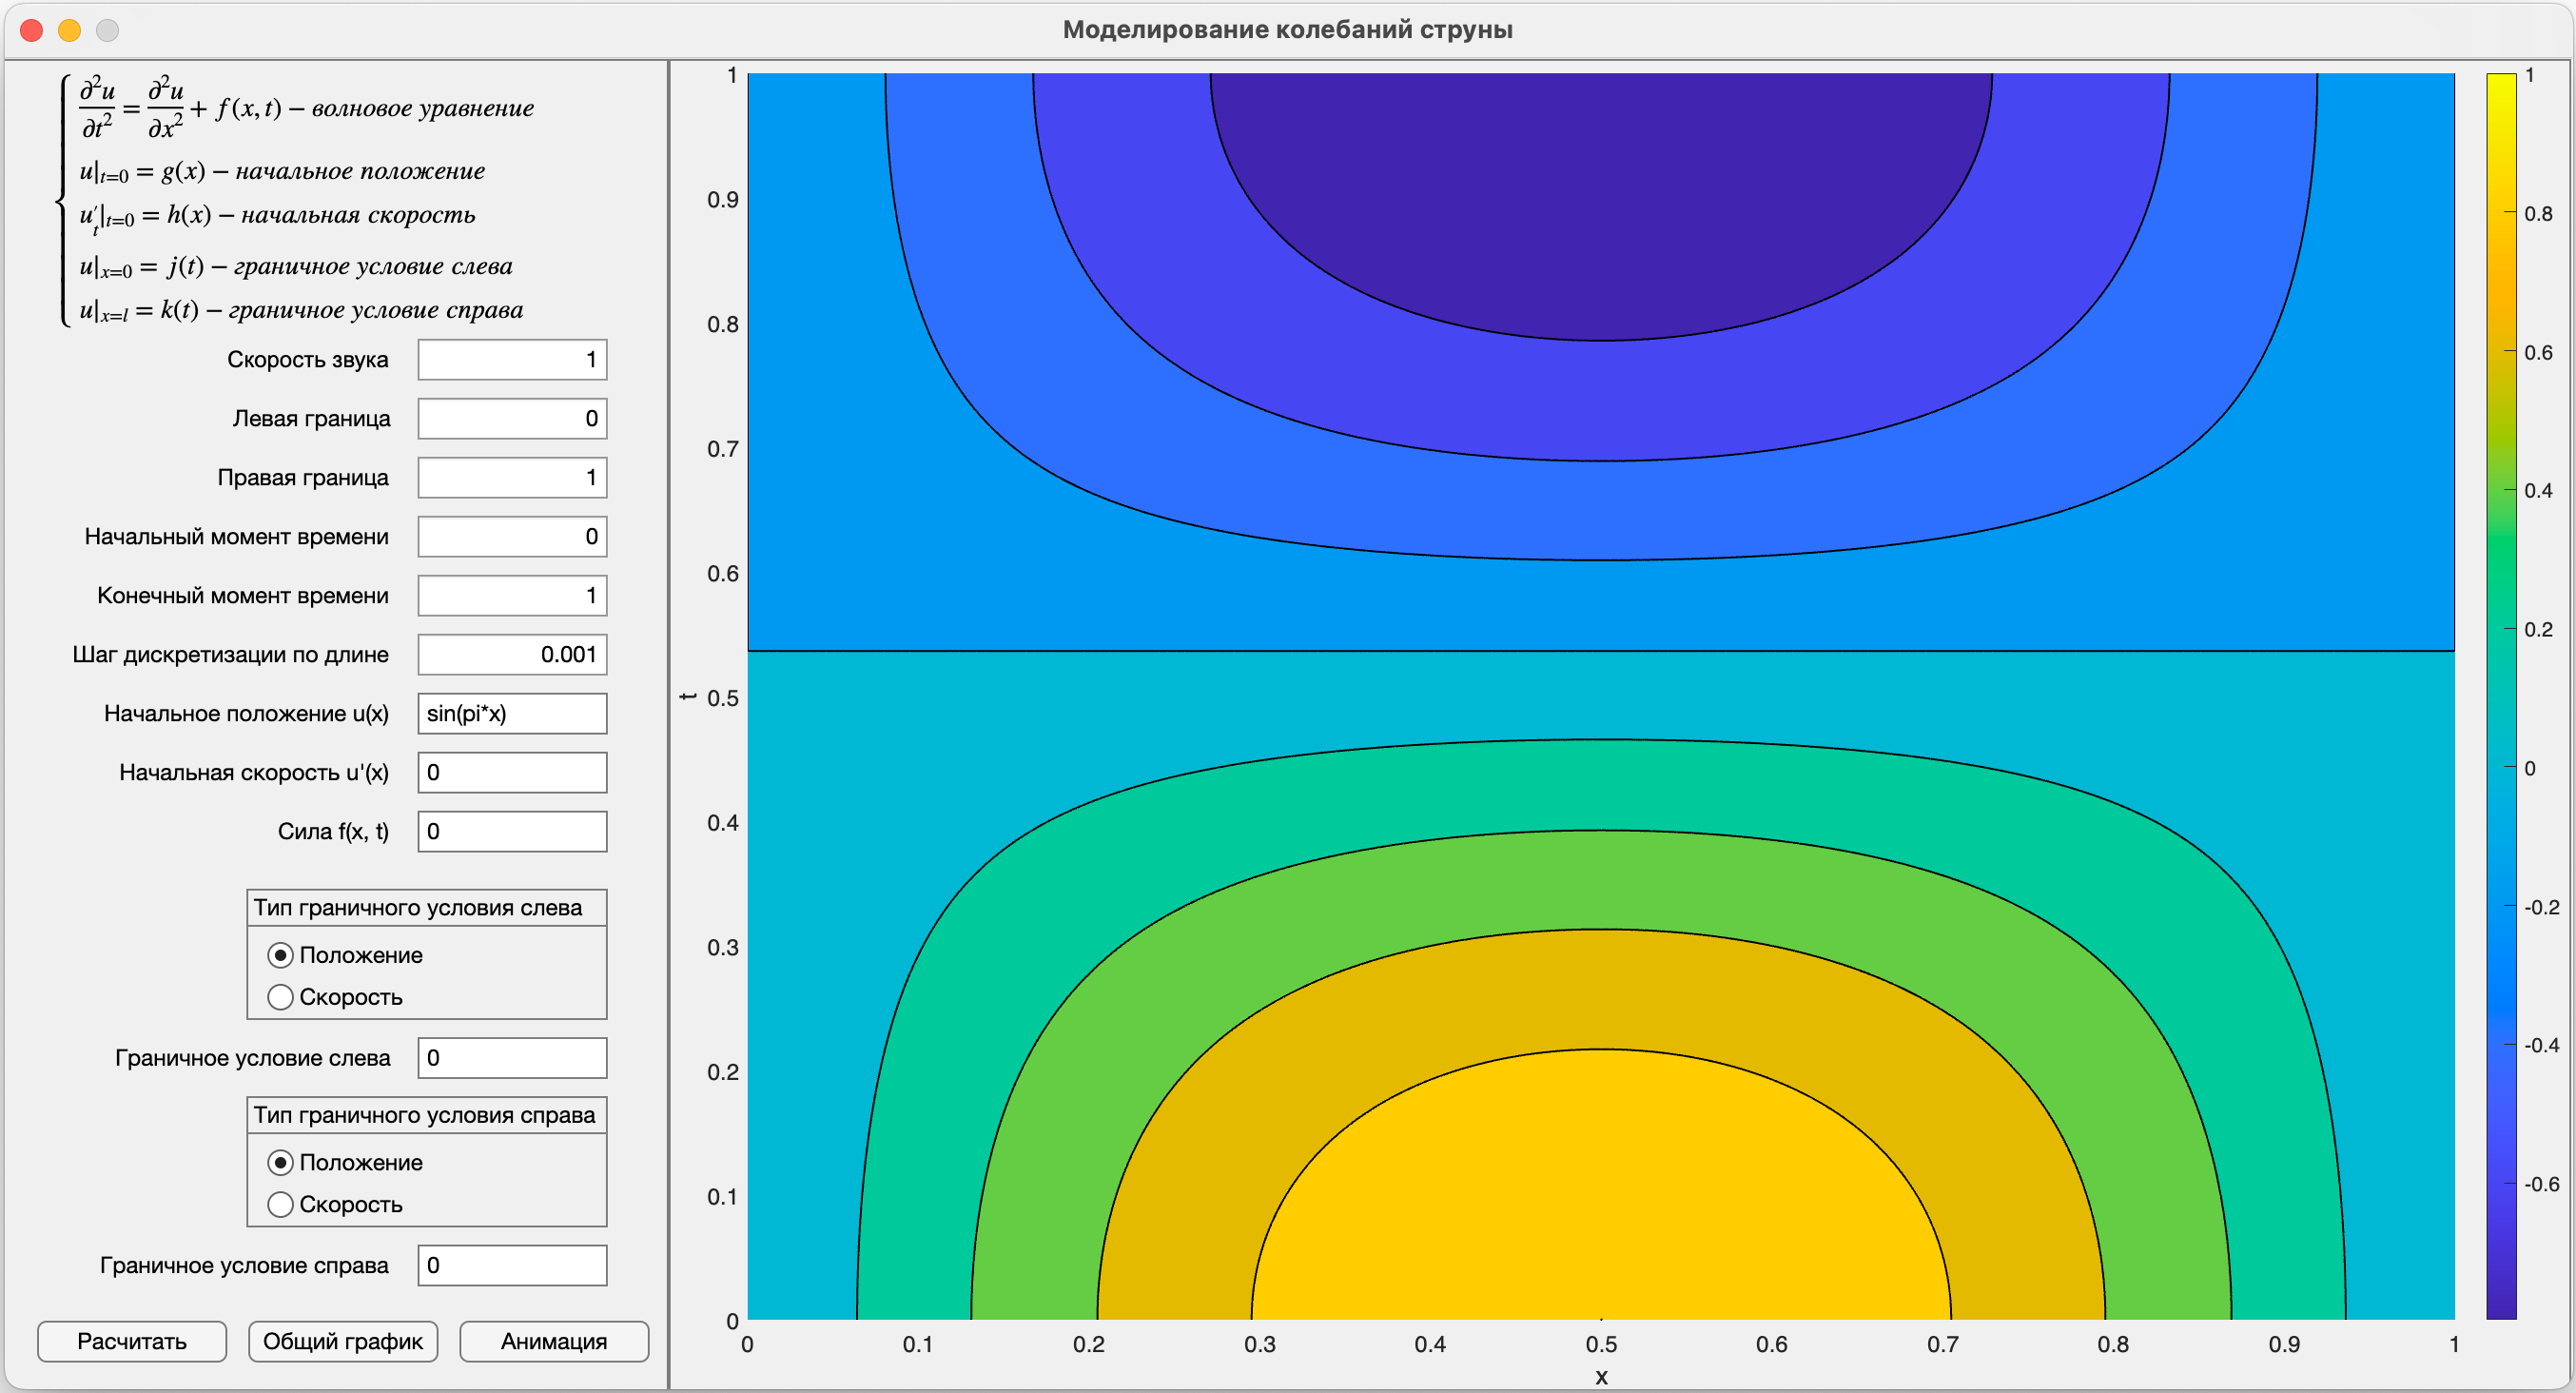
\includegraphics[width=1\linewidth]{Wave eqation/program.png}}
	 	\caption{Рабочее окно программы.}
	 	\label{img:program}
	 \end{figure}
	 
	 Окно разделено на 2 части: слева пользователем вводятся условия задачи, а справа отображается график решения.
	 
	 Пользователь указывает:
	 \begin{itemize}
	 	\item скорость звука;
	 	\item начальное и конечное значения координаты;
	 	\item начальное и конечное значения времени;
	 	\item шаг дискретизации по длине;
	 	\item функции начального положения и скорости;
	 	\item функцию внешней силы, которая может зависеть как от координат, так и от времени;
	 	\item типы граничных условий (координата или скорость) и функции соответствующих условий.
	 \end{itemize}
	 
	 Под полями с условиями расположены три кнопки:
	 \begin{itemize}
	 	\item Рассчитать \\
	 	По нажатию на эту кнопку происходит расчёт значений по аналогии со скриптовым вариантом.
	 	
	 	\item  Общий график \\
	 	После нажатия происходит построение графика в координатах $(x, t)$, где за функцию $u(x, t)$ отвечает цвет в соответствующей точке.
	 	
	 	\item Анимация \\
	 	По нажатию начинается анимация положения струны.
	 \end{itemize}
	 
	 \subsubsection{Программа для решения уравнения колебаний прямоугольной мембраны}
	
	В случае с колебанием двумерной прямоугольной мембраны написан только скрипт c использованием Partial Differential Equation Toolbox \cite{MathWorks_PDEToolbox}.
	
	В скрипте пользователь указывает:
	\begin{itemize}
		\item скорость звука;
		\item начальное и конечное значения координат;
		\item начальное и конечное значения времени;
		\item шаг дискретизации по времени;
		\item размер конечного элемента;
		\item функции начального положения и скорости;
		\item функцию внешней силы, которая может зависеть как от координат, так и от времени;
		\item функции граничных условий.
	\end{itemize}
	
	Весь скрипт разделен на фрагменты, в каждом из которых выполняется одно действие. Также добавлена возможность вывести изображения геометрии задачи и построенной сетки для промежуточного контроля.
	Общий алгоритм работы скрипта:
	
	\begin{enumerate}
		\item создание модели PDE;
		\item задание геометрии, типа уравнения, коэффициентов уравнения, начальных и граничных условий;
		\item построение сетки;
		\item численное решение уравнения;
		\item построение графика решения.
	\end{enumerate}
	
	\newpage
	\subsection{Результаты расчётов для разных условий}
	
	% условия - картинка
	
	\subsubsection{Условия по-умолчанию}
	
	Для демонстрации работы программы при запуске поля заполнены следующими условиями:
	
	\begin{equation*}
		\left\{\begin{array}{@{}l@{}}
			\displaystyle \frac{\partial^2u}{\partial t^2} = c^2 \cdot \frac{\partial^2u}{\partial x^2}; \\
			x_{min} = 0; \; x_{max} = 1; \\
			 t_{min} = 0; \; t_{max} = 1; \\
			 c = 1; \;  \Delta x = 0.001; \\
			u|_{t=0} = \sin \pi x; \\
			u'_{t}|_{t=0} = 0; \\
			u|_{x=0} = 0; \\
			u|_{x=1} = 0.
		\end{array}\right.\,
	\end{equation*}
	
	Результат решения изображен на рисунке \ref{img:first_task}.
	
	\begin{figure}[h]
		\center{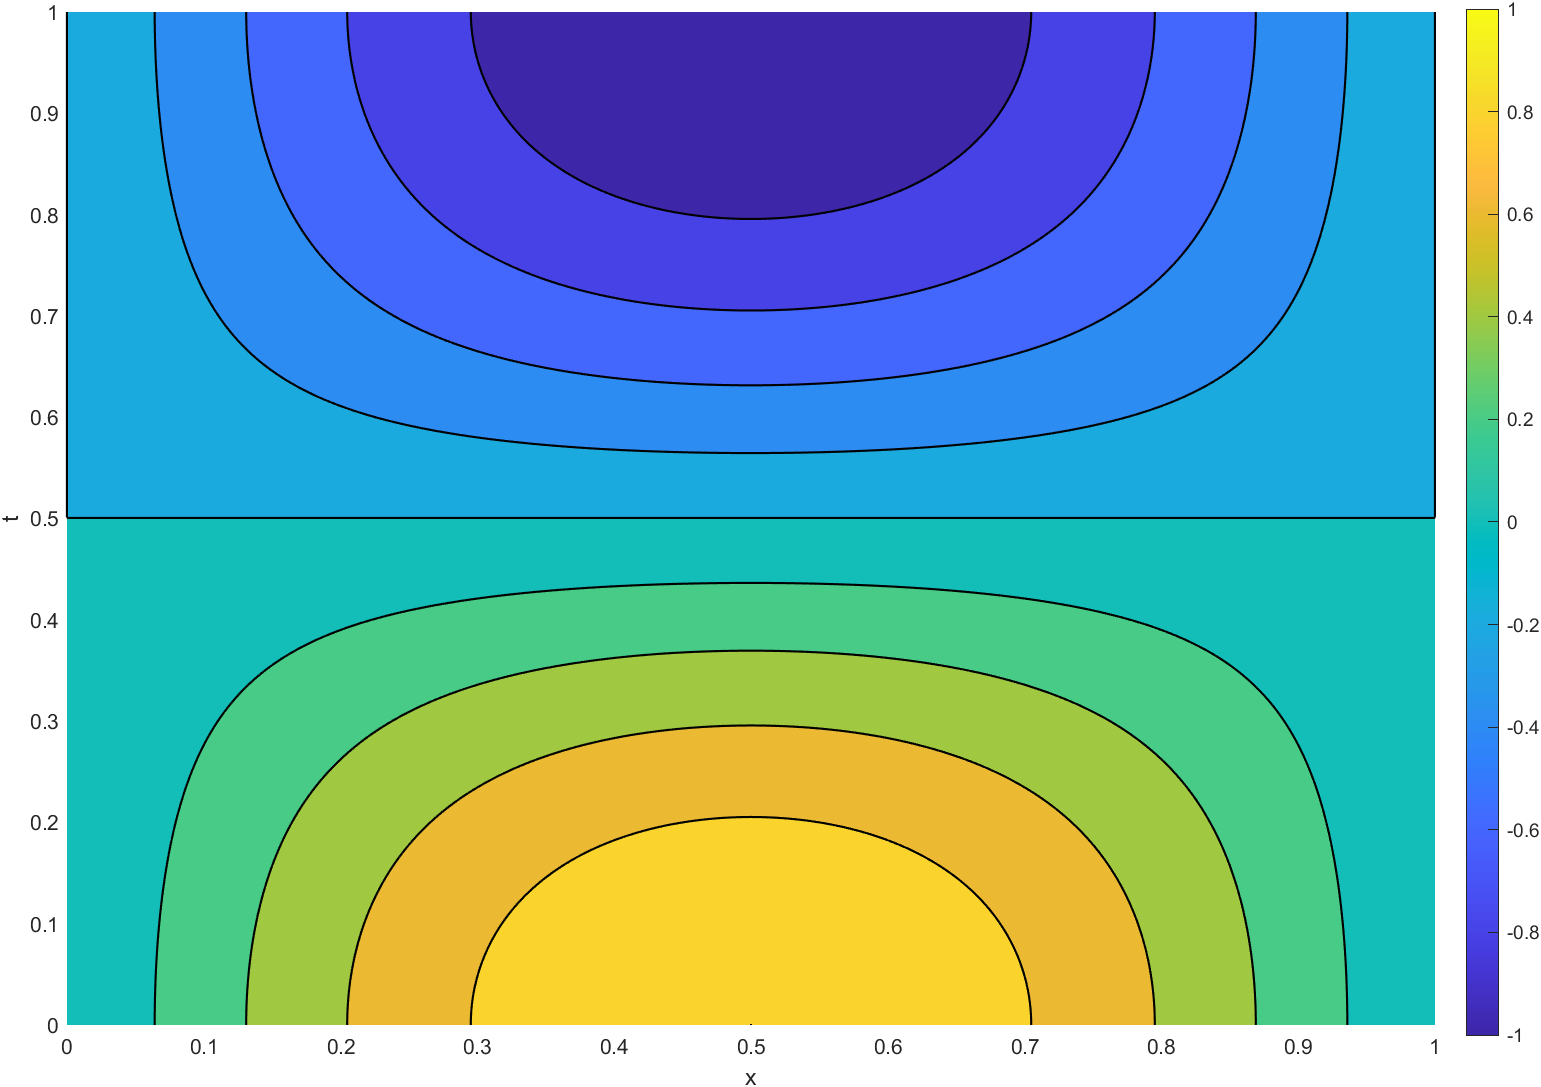
\includegraphics[width=1\linewidth]{Wave eqation/1.png}}
		\caption{Решение первой задачи.}
		\label{img:first_task}
	\end{figure}
	
	Полученный результат совпадает с аналитическим решением с максимальным отклонением 0,015, когда струна проходит положение равновесия. В среднем относительная погрешность равна 5\%.
	
	\newpage
	\subsubsection{Положение равновесия с начальной скоростью}
	
	Вместо начального положения зададим начальную скорость:
	
	\begin{equation*}
		\left\{\begin{array}{@{}l@{}}
			\displaystyle \frac{\partial^2u}{\partial t^2} = c^2 \cdot \frac{\partial^2u}{\partial x^2}; \\
			x_{min} = 0; \; x_{max} = 1; \\
			t_{min} = 0; \; t_{max} = 1; \\
			c = 1; \;  \Delta x = 0.001; \\
			u|_{t=0} = 0; \\
			u'_{t}|_{t=0} = \sin \pi x; \\
			u|_{x=0} = 0; \\
			u|_{x=1} = 0.
		\end{array}\right.\,
	\end{equation*}
	
	Результат решения изображен на рисунке \ref{img:second_task}.
	
	\begin{figure}[h]
		\center{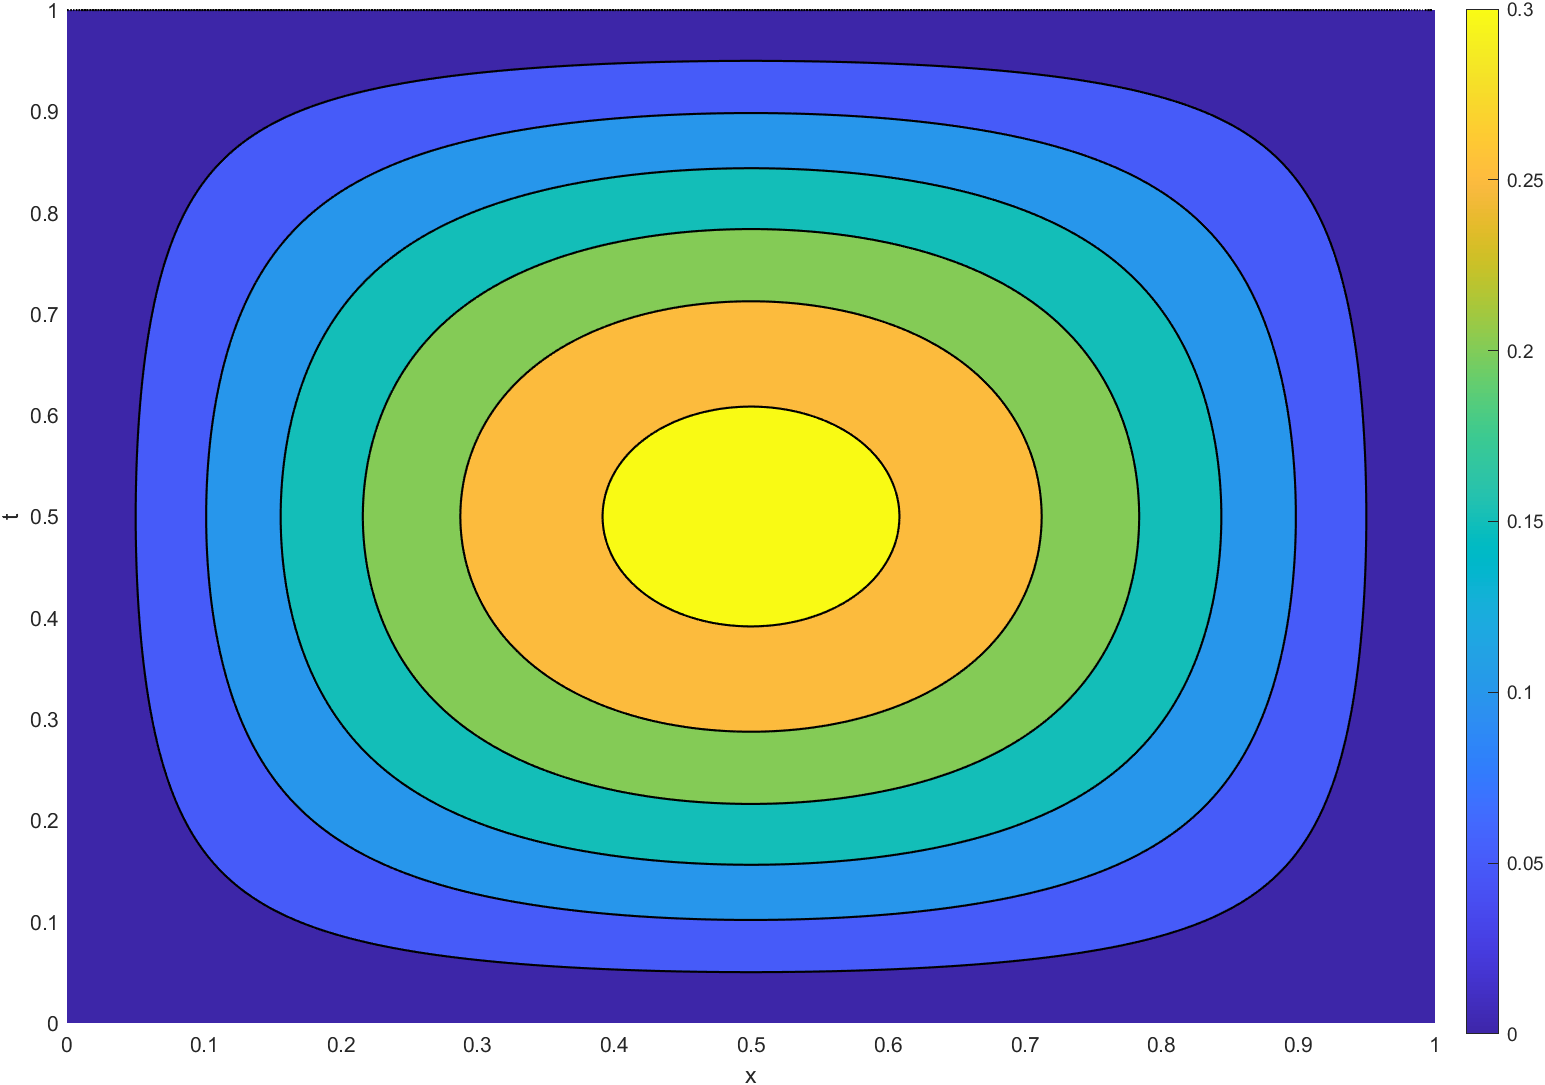
\includegraphics[width=1\linewidth]{Wave eqation/2.png}}
		\caption{Решение второй задачи.}
		\label{img:second_task}
	\end{figure}
	
	\newpage
	\subsubsection{Резонанс струны}
	
	Приложим к струне силу, меняющуюся с частотой первой гармоники струны:
	
	\begin{equation*}
		\left\{\begin{array}{@{}l@{}}
			\displaystyle \frac{\partial^2u}{\partial t^2} = c^2 \cdot \frac{\partial^2u}{\partial x^2} + \sin \pi x \cdot \sin \pi t; \\
			x_{min} = 0; \; x_{max} = 1; \\
			t_{min} = 0; \; t_{max} = 5; \\
			c = 1; \;  \Delta x = 0.001; \\
			u|_{t=0} = 0; \\
			u'_{t}|_{t=0} = 0; \\
			u|_{x=0} = 0; \\
			u|_{x=1} = 0.
		\end{array}\right.\,
	\end{equation*}
	
	Результат решения изображен на рисунке \ref{img:third_task}. Видно, что амплитуда колебаний увеличивается со временем.
	
	\begin{figure}[h]
		\center{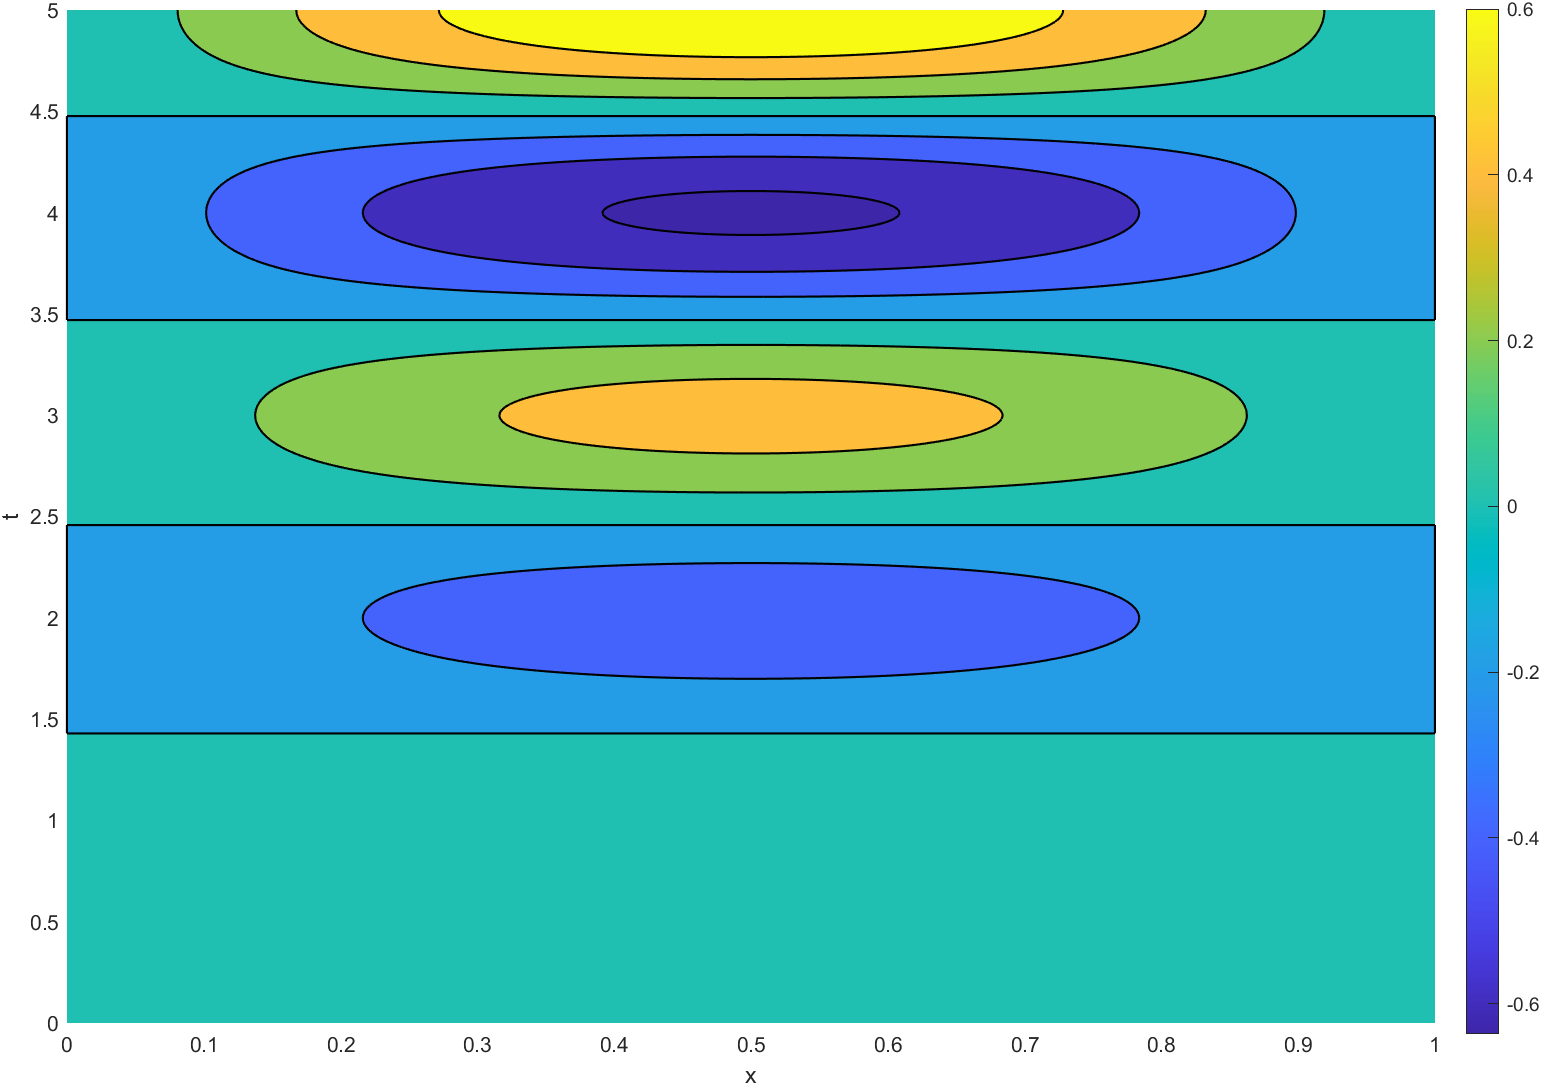
\includegraphics[width=1\linewidth]{Wave eqation/3.png}}
		\caption{Решение третьей задачи.}
		\label{img:third_task}
	\end{figure}
	
	\newpage
	\subsubsection{Сумма трёх гармоник}
	
	Смоделируем колебание струны на первых трёх собственных частотах:
	
	\begin{equation*}
		\left\{\begin{array}{@{}l@{}}
			\displaystyle \frac{\partial^2u}{\partial t^2} = c^2 \cdot \frac{\partial^2u}{\partial x^2}; \\
			x_{min} = 0; \; x_{max} = 1; \\
			t_{min} = 0; \; t_{max} = 1; \\
			c = 1; \;  \Delta x = 0.001; \\
			u|_{t=0} = 0; \\
			u'_{t}|_{t=0} = 0; \\
			u|_{x=0} = \sin 3 \pi t; \\
			u|_{x=1} = 0.
		\end{array}\right.\,
	\end{equation*}
	
	Результат решения изображен на рисунке \ref{img:fourth_task}.
	
	\begin{figure}[h]
		\center{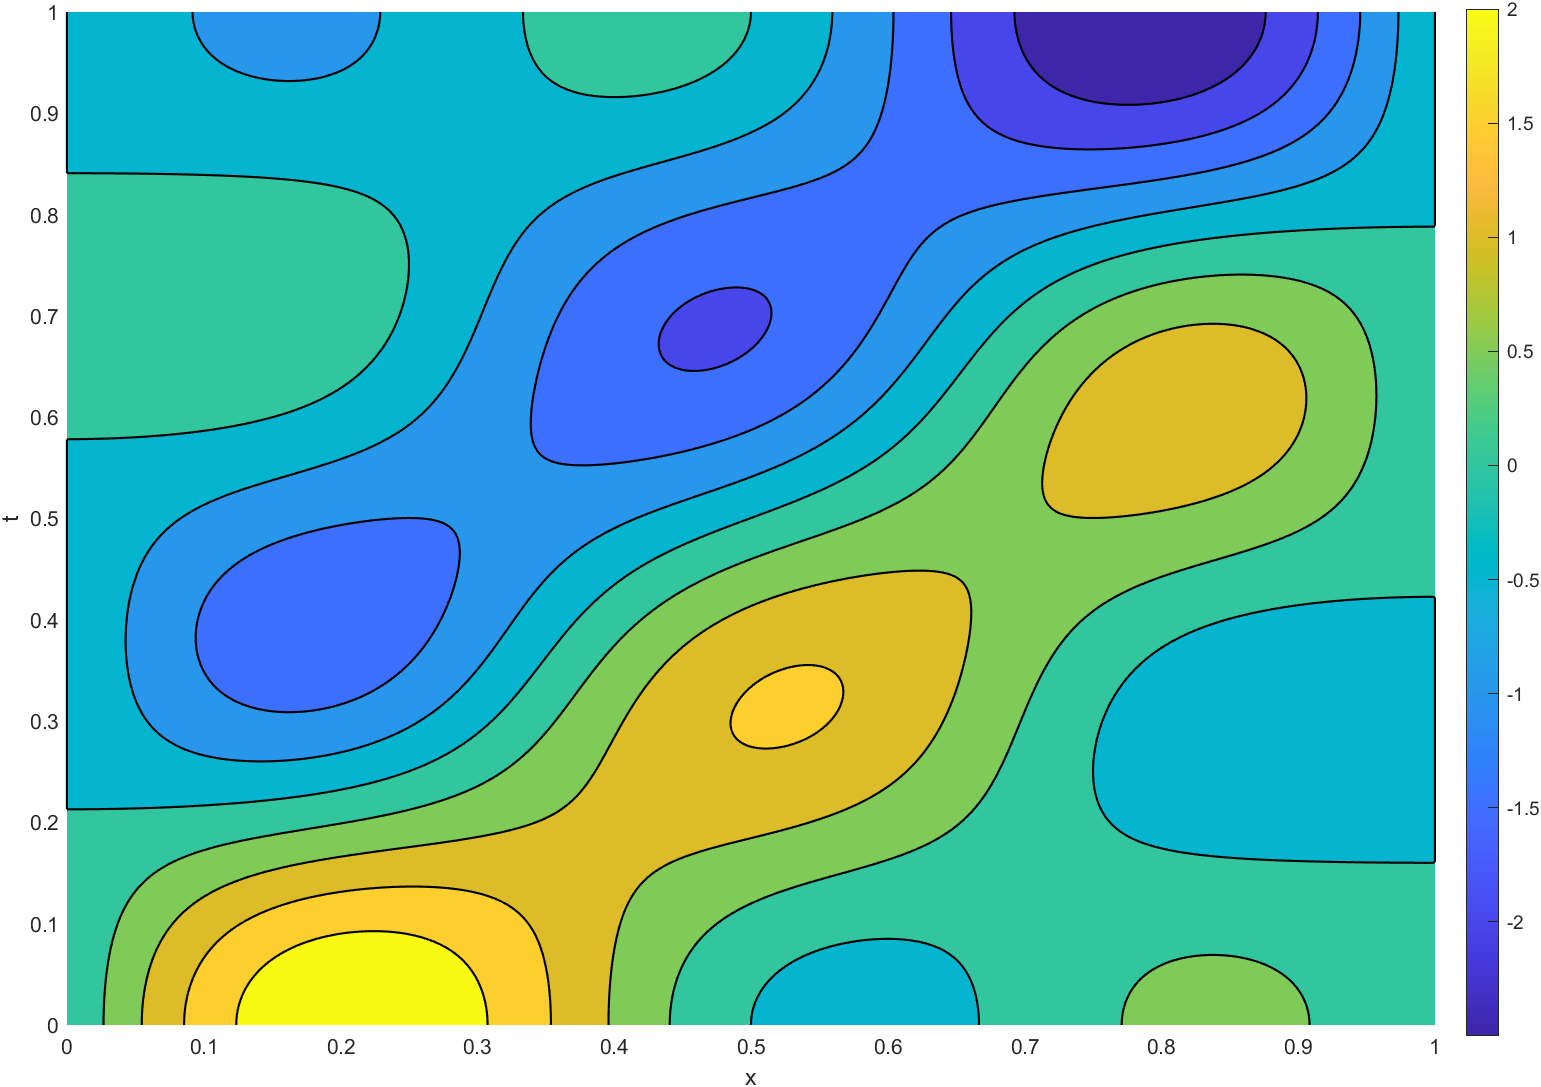
\includegraphics[width=1\linewidth]{Wave eqation/4.png}}
		\caption{Решение четвертой задачи.}
		\label{img:fourth_task}
	\end{figure}
	
	\newpage
	\subsubsection{Колебание одного края струны}
	
	Смоделируем струну, край которой движется по гармоническому закону:
	
	\begin{equation*}
		\left\{\begin{array}{@{}l@{}}
			\displaystyle \frac{\partial^2u}{\partial t^2} = c^2 \cdot \frac{\partial^2u}{\partial x^2}; \\
			x_{min} = 0; \; x_{max} = 1; \\
			t_{min} = 0; \; t_{max} = 5; \\
			c = 1; \;  \Delta x = 0.001; \\
			u|_{t=0} = \sin \pi x + \sin 2 \pi x + \sin 3 \pi x; \\
			u'_{t}|_{t=0} = 0; \\
			u|_{x=0} = 0; \\
			u|_{x=1} = 0.
		\end{array}\right.\,
	\end{equation*}
	
	Результат решения изображен на рисунке \ref{img:fifth_task}. Видно как распространяется волна по струне, отражается от правого края и интерферирует сама с собой, образуя стоячую волну.
	
	\begin{figure}[h]
		\center{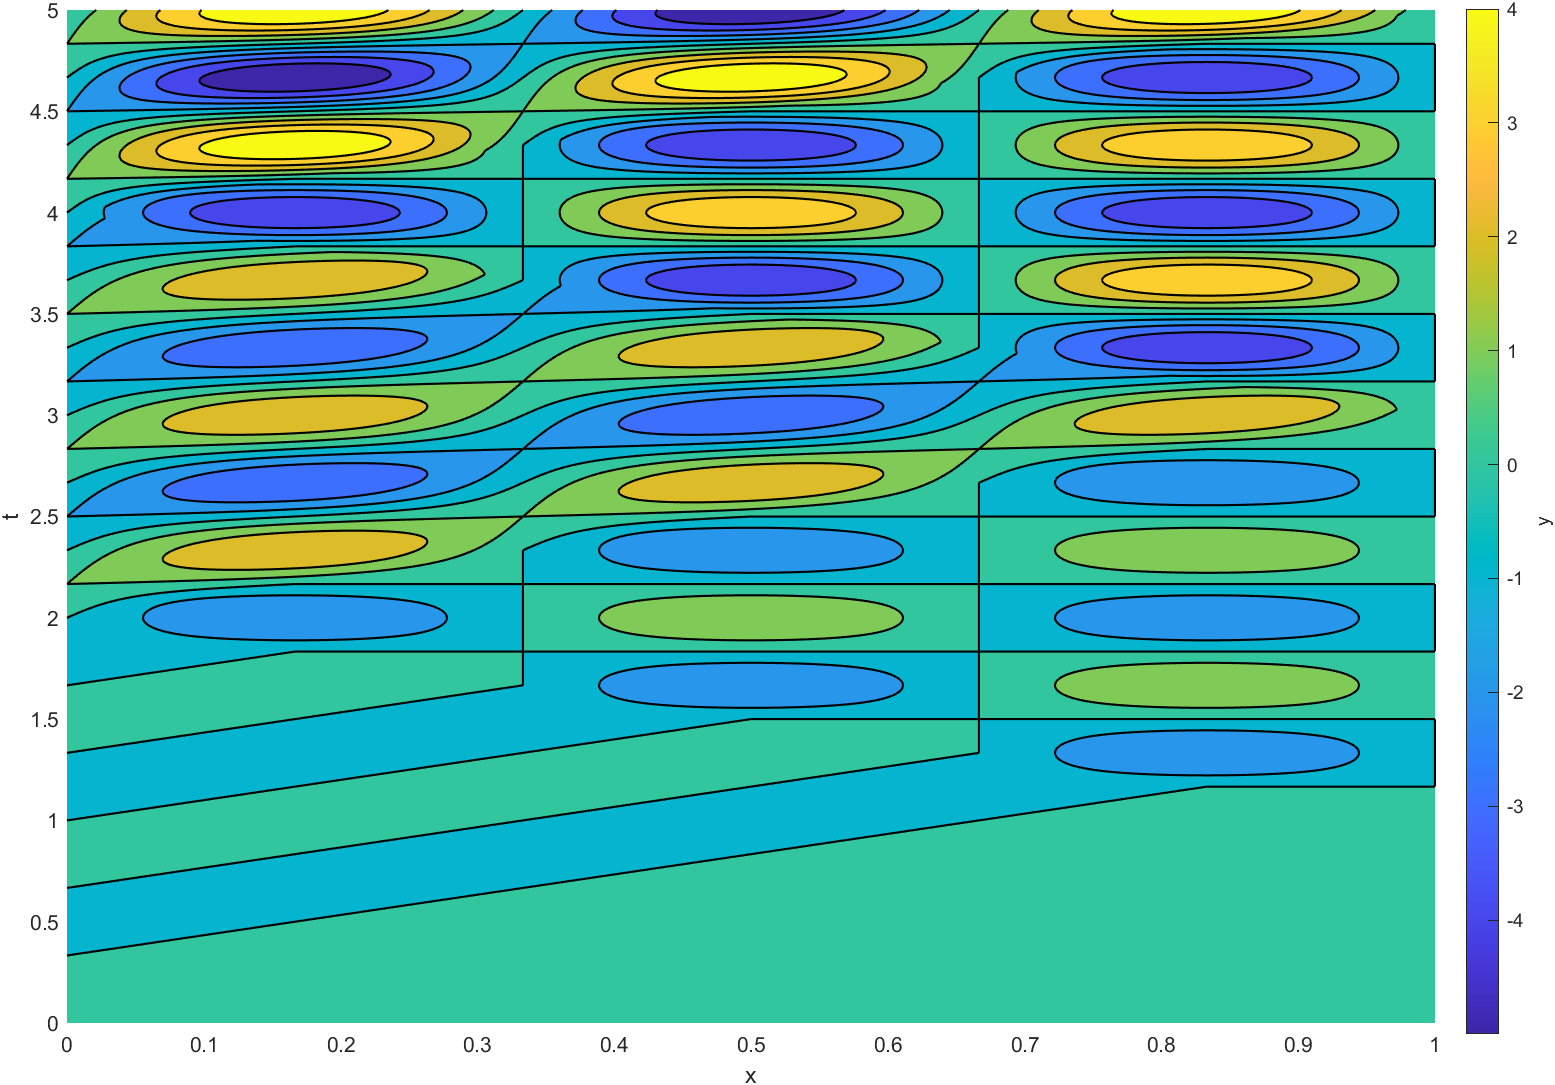
\includegraphics[width=1\linewidth]{Wave eqation/5.png}}
		\caption{Решение пятой задачи.}
		\label{img:fifth_task}
	\end{figure}
	
	\newpage
	\subsubsection{Колебание одного края струны}
	
	Смоделируем струну, край которой движется по гармоническому закону:
	
	\begin{equation*}
		\left\{\begin{array}{@{}l@{}}
			\displaystyle \frac{\partial^2u}{\partial t^2} = c^2 \cdot \frac{\partial^2u}{\partial x^2}; \\
			x_{min} = 0; \; x_{max} = 1; \\
			t_{min} = 0; \; t_{max} = 5; \\
			c = 1; \;  \Delta x = 0.001; \\
			u|_{t=0} = \sin \pi x + \sin 2 \pi x + \sin 3 \pi x; \\
			u'_{t}|_{t=0} = 0; \\
			u|_{x=0} = 0; \\
			u|_{x=1} = 0.
		\end{array}\right.\,
	\end{equation*}
	
	Результат решения изображен на рисунке \ref{img:fifth_task}. Видно как распространяется волна по струне, отражается от правого края и интерферирует сама с собой, образуя стоячую волну.
	
	\begin{figure}[h]
		\center{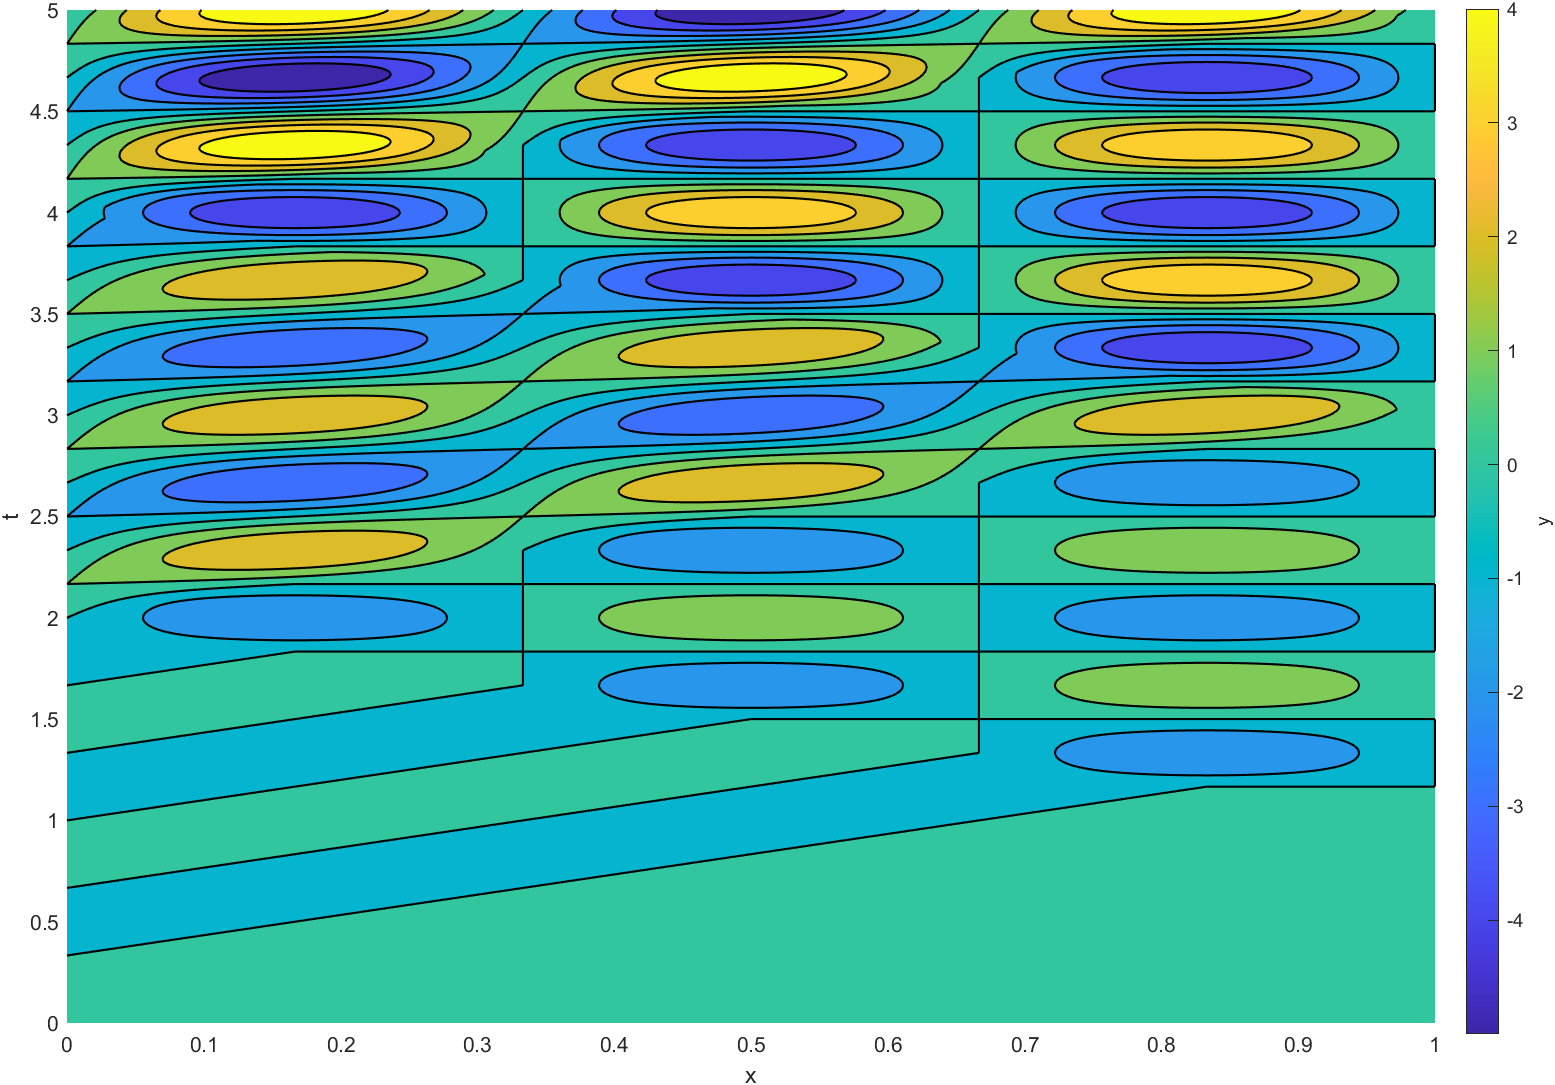
\includegraphics[width=1\linewidth]{Wave eqation/5.png}}
		\caption{Решение пятой задачи.}
		\label{img:fifth_task}
	\end{figure}
	


	\newpage
	\makeatletter
	\addcontentsline{toc}{chapter}{СПИСОК ИСПОЛЬЗОВАННЫХ ИСТОЧНИКОВ И ЛИТЕРАТУРЫ}
	\refstepcounter{chapter}
	\begin{thebibliography}{99}
		
		\bibitem{Diep1} Львовский С. Набор и вёрстка в системе LATEX. -- 5-е изд., переработанное. -- М.: МЦНМО, 2014. -- 400 с
		
		
		
		
		\bibitem{Tihonov_Urmatfiz} Тихонов А. Н., Самарский А. А. Уравнения математической физики: Учебное пособие. -- 6-е изд., испр. и доп. -- М.: Изд-во МГУ, 1999. -- 798 с. -- ISBN 5-211-04138-0.
		\bibitem{Panov_MathPhys} Панов Ю. Д., Егоров Р. Ф. Математическая физика. Методы решения задач -- Екатеринбург: Изд-во УрГУ, 2005. -- 150 с.
		\bibitem{Priklonski_NumMethods} Приклонский В. И., Ульянова Л. Численные методы в физике. Конспект лекций. -- 130 с.
		\bibitem{Semenchok_String} Семченок М. С., Щитов И. Н. Колебания струны: Методическое пособие. -- СПб: СПбГИКиТ, 2010 -- 43 с.
		\bibitem{Gallager_MKE} Галлагер Р. Метод конечных элементов. Основы: Пер. с англ. — М.: Мир, 1984
		\bibitem{Samarski_SetochMethods} Самарский А. А., Николаев Е. С. Методы решения сеточных уравнений. — Москва: Наука, 1978. — 592 с.
		\bibitem{Diakonov_MATLAB} Дьяконов В. П. MATLAB. Полный самоучитель. — Москва: ДМК Пресс, 2012. — 768 с.: ил.
		\bibitem{MathWorks_PDEToolbox} Partial Differential Equation Toolbox User's Guide — The MathWorks, 2016. — 904 с.
		\bibitem{MathWorks_AppBuilding} MATLAB App Building — The MathWorks, 2023. — 490 с.
		
	\end{thebibliography}
	
\end{document}


